\documentclass[a4paper]{report}
\usepackage[utf8]{vietnam}
\usepackage[utf8]{inputenc}
\usepackage{amsmath}
\usepackage{amsfonts}
\usepackage{amssymb}
\usepackage{graphicx}
\usepackage{xspace}
\usepackage[font=small]{caption}
\usepackage{booktabs}
\usepackage[unicode]{hyperref}
\usepackage[left=3cm,right=2cm,top=2.5cm,bottom=3cm]{geometry}
\usepackage{titlesec}
\usepackage{scrextend}
\usepackage{enumerate}
\usepackage{url}
\usepackage{tikz}
\usepackage{float}
\usepackage{afterpage}
\usepackage{multirow}
\usepackage{sectsty}
\usepackage{tocloft,calc}
\usepackage{listings}
\usepackage{makecell}
\usepackage[numbers,sort&compress]{natbib}
\usetikzlibrary{calc}
\usepackage{algorithm}
\usepackage{subcaption}
\usepackage{amsthm}
\usepackage{enumitem}
\usepackage{mdframed}
\usepackage[flushleft]{threeparttable}
\usepackage{perpage}
\newtheorem{definition}{Definition}[chapter]

\MakePerPage{footnote}
\PassOptionsToPackage{table}{xcolor}

\def\changemargin#1#2{\list{}{\rightmargin#2\leftmargin#1}\item[]}
\let\endchangemargin=\endlist

\changefontsizes{13pt}
\bibliographystyle{unsrtnat}

\makeatletter
\def\l@figure{\@dottedtocline{1}{1em}{2.2em}}
\def\l@table{\@dottedtocline{1}{1em}{2.2em}}
\renewcommand*{\ALG@name}{Algorithm}
\gdef\@chapapp{Chapter}
\makeatother

\sectionfont{\fontsize{15}{15}\selectfont}
\subsectionfont{\fontsize{13}{15}\selectfont}

\titleformat{\chapter}[display]
{\normalfont\huge\bfseries}{\chaptertitlename\ \thechapter}{0pt}{\LARGE}
\titlespacing*{\chapter}{0cm}{-\topskip}{0pt}[0pt]

\renewcommand{\baselinestretch}{1.3}
\renewcommand{\chaptername}{Chapter}
\renewcommand{\chaptertitlename}{Chapter}
\renewcommand{\contentsname}{Contents}
\renewcommand{\listfigurename}{List of Figures}
\renewcommand{\listtablename}{List of Tables}
\renewcommand{\figurename}{Figure}
\renewcommand{\tablename}{Table}
\renewcommand{\bibname}{References}
\renewcommand{\cftchappresnum}{Chapter }
\AtBeginDocument{\addtolength\cftchapnumwidth{\widthof{\bfseries Chapter }}}
\setlength{\parskip}{0.4em}
\setlength{\parindent}{0pt}

\title{Antimicrobial Resistance Prediction from Bacterial Genome}
\author{Mạc Gia Khánh and Đào Xuân Nghĩa}

\newcommand{\argmax}{\arg\!\max}
\newcommand{\tool}{\textsc{ToolName}\xspace}
\newcommand{\modulea}{\textit{ModuleA}\xspace}
\newcommand{\moduleb}{\textit{ModuleB}\xspace}
\newcommand{\frameworka}{\textsc{FrameworkA}\xspace}
\newcommand{\dataseta}{\textsc{DatasetA}\xspace}
\newcommand{\datasetb}{\textsc{DatasetB}\xspace}
\newcommand{\toolLong}{\textbf{Long Tool Name}\xspace}
\newcommand{\methoda}{\textit{MethodA}\xspace}
\newcommand{\methodb}{\textit{MethodB}\xspace}
\newcommand{\baselinea}{\textit{BaselineA}\xspace}

\definecolor{dkgreen}{rgb}{0,0.6,0}
\definecolor{gray}{rgb}{0.5,0.5,0.5}
\definecolor{mauve}{rgb}{0.58,0,0.82}
\definecolor{darkblue}{rgb}{0.0,0.0,0.6}
\definecolor{lightblue}{rgb}{0.0,0.0,0.9}
\definecolor{cyan}{rgb}{0.0,0.6,0.6}
\definecolor{darkred}{rgb}{0.6,0.0,0.0}
\definecolor{bg_gray}{RGB}{242, 242, 235}

\renewcommand{\lstlistingname}{Listing}
\newcommand{\cev}[1]{\reflectbox{\ensuremath{\vec{\reflectbox{\ensuremath{#1}}}}}}

\lstset{
  basicstyle=\ttfamily\footnotesize,
  columns=fullflexible,
  showstringspaces=false,
  numbers=left,
  numberstyle=\small\color{gray},
  stepnumber=1,
  numbersep=5pt,
  backgroundcolor=\color{bg_gray},
  showspaces=false,
  showtabs=false,
  frame=none,
  rulecolor=\color{black},
  tabsize=2,
  captionpos=b,
  breaklines=true,
  breakatwhitespace=false,
  title=\lstname,
  commentstyle=\color{gray}\upshape
}

\usepackage[table]{xcolor}
\definecolor{light-gray}{gray}{0.92}

\begin{document}
\hypersetup{pageanchor=false}
\pagenumbering{gobble}

\begin{center}
    \begin{tikzpicture}[overlay,remember picture]
    \draw [line width=3pt,rounded corners=0pt]
    ($ (current page.north west) + (25mm,-25mm) $)
    rectangle
    ($ (current page.south east) + (-15mm,25mm) $);
    \draw [line width=1pt,rounded corners=0pt]
    ($ (current page.north west) + (26.5mm,-26.5mm) $)
    rectangle
    ($ (current page.south east) + (-16.5mm,26.5mm) $);
    \end{tikzpicture}
    \\[1mm]
    \textbf{UNIVERSITY NAME\\FACULTY OR SCHOOL}
    \\[1cm]
    
\includegraphics[width=0.2\linewidth]{figures/uet}
    \\[0.3cm]
    \textbf{STUDENT NAME \\
    STUDENT ID}
    \\[2cm]

    \large{\textbf{THESIS TITLE}}
    \\[2.6cm]
    \normalsize{\textbf{THESIS TYPE
        \\[2mm]
    MAJOR}}
\end{center}
\vspace{16mm}
\hspace*{12mm}\textbf{Supervisor: SUPERVISOR NAME}\\[0.8cm]
\vfill
\begin{center}
    \textbf{CITY - YEAR}
    \vspace{10mm}
\end{center}
\newpage\cleardoublepage
\chapter*{Abstract}
\addcontentsline{toc}{chapter}{Abstract}

This report presents a determinant-based workflow for predicting antimicrobial resistance in \textit{Salmonella enterica} from bacterial genomic data. The main objective is to determine whether curated resistance determinants, including acquired resistance genes and resistance-associated mutations, can be used to predict binary resistant/susceptible phenotypes for individual antibiotics. Instead of relying on genome-wide feature spaces that are harder to interpret biologically, the study focuses on a curated determinant space derived from AMRFinderPlus and MicroBIGG-E.

The workflow has three main parts: cleaning phenotype labels from AST data, cleaning and normalizing genotype records, and building one model-ready table for each antibiotic. To study how much biological knowledge should be used before learning starts, the report compares three connection scopes: \textit{strict}, \textit{broad}, and \textit{all}. XGBoost models are then trained for each antibiotic with five-fold cross-validation. In addition, two simple rule-based baselines, \textit{strict rule-based} and \textit{broad rule-based}, are used as direct references without machine learning.

The results show that \textit{all ML} gives the best overall predictive performance, while \textit{broad ML} gives the best balance between feature coverage and biological interpretability. The rule-based baselines also show that, for some antibiotics, known genes and mutations are already enough for very accurate prediction. For other antibiotics, however, this direct gene-to-label rule is too simple and produces many false positives or false negatives. In those cases, machine learning helps by combining several signals at the same time.

Overall, the study shows that AMR prediction from curated genes and mutations is a suitable bioinformatics approach for this problem. It also shows that the difference between \textit{strict}, \textit{broad}, and \textit{all} is important: these settings represent different trade-offs between biological simplicity, ease of interpretation, and predictive accuracy.
\newpage\cleardoublepage
% \chapter*{Abstract (English)}
\addcontentsline{toc}{chapter}{Abstract (English)}

Replace this section with the English abstract.
\newpage\cleardoublepage
\renewcommand{\contentsname}{Contents}
\addcontentsline{toc}{chapter}{Contents}
\tableofcontents\newpage\cleardoublepage

\newpage
\renewcommand{\listfigurename}{List of Figures}
\addcontentsline{toc}{chapter}{List of Figures}
\listoffigures\cleardoublepage

\newpage
\renewcommand{\listtablename}{List of Tables}
\addcontentsline{toc}{chapter}{List of Tables}
\listoftables

\newpage
\chapter*{Glossary}
\addcontentsline{toc}{chapter}{Glossary}

\begin{tabular}{|m{3cm}|m{10cm}|}
\hline
\textbf{Term} & \textbf{Description} \\ \hline
Example & Replace with your glossary entries. \\ \hline
\end{tabular}
\newpage\cleardoublepage

\hypersetup{pageanchor=true}
\setcounter{page}{1}
\pagenumbering{arabic}

\chapter{Chapter 1 Title}

\section{Problem Statement}

Replace this section with your problem statement.

\section{Related Work}

Replace this section with your related work.

\section{Objectives}

Replace this section with your objectives.

\newpage\cleardoublepage
\chapter{Biological Background and Data Description}

\section{Biological background of antimicrobial resistance}

Antimicrobial resistance appears when bacteria gain genetic changes that weaken or block the effect of an antibiotic. In practice, these changes are often known resistance genes or specific mutations. In \textit{Salmonella enterica}, resistance can come from several well-known mechanisms, for example enzymes that break down beta-lactam drugs such as penicillins and cephalosporins, genes that protect against tetracycline, or mutations linked to quinolone resistance.

For this reason, AMR prediction from genomic data is not only a classification task. It is also an interpretation task. A useful AMR predictor should not only output a label, but should also keep a clear link between that label and known resistance genes or mutations.

\section{Phenotype definition: AST and resistance labels}

The phenotype side of the project comes from antimicrobial susceptibility testing. AST checks whether an isolate behaves as resistant or susceptible to a specific drug in laboratory conditions. The raw measurement is often the minimum inhibitory concentration (MIC), which is the drug level needed to stop visible bacterial growth. This value is then converted into a label such as susceptible, intermediate, or resistant according to a breakpoint standard.

In this project, the final supervised learning label is binary:

\begin{itemize}
    \item \textbf{Resistant} is encoded as the positive class.
    \item \textbf{Susceptible} is encoded as the negative class.
\end{itemize}

Intermediate, nonstandard, and ambiguous labels are excluded to avoid adding noise near the decision boundary. This choice fits the present study because the goal is a robust binary prediction task rather than detailed MIC prediction.

\section{Genotype definition: curated AMR determinants}

The genotype side of the project is built from curated AMR determinant resources rather than raw sequence fragments. Each isolate is represented by detected resistance genes and mutations reported by AMRFinderPlus and organized in the MicroBIGG-E resource. This is useful because AMRFinderPlus provides a curated catalog and structured annotations for resistance determinants~\citep{feldgarden2021amrfinderplus}. Each determinant record contains several important fields:

\begin{itemize}
    \item \texttt{Element symbol}: the name of the gene or mutation.
    \item \texttt{Class}: a broad drug class.
    \item \texttt{Subclass}: a more specific drug group.
    \item \texttt{Subtype}: whether the determinant is a gene or a mutation.
    \item \texttt{Method}: how the determinant was detected.
    \item \texttt{Scope}: how conservative the evidence is.
\end{itemize}

This representation is appropriate because every feature still has a biological meaning and can be traced back to a known resistance mechanism.

\section{Data sources used in the project}

The project uses three major data sources:

\begin{enumerate}[label=\arabic*.]
    \item \textbf{Assembled genomes in FASTA format}, used for AMRFinderPlus-based prototype validation.
    \item \textbf{NCBI MicroBIGG-E genotype data}, used as the main large-scale determinant table for feature construction.
    \item \textbf{NCBI AST phenotype data}, used as the ground-truth source of antibiotic resistance labels.
\end{enumerate}

The common key connecting these resources is the \texttt{BioSample} identifier. It allows genotype and phenotype rows to be matched isolate by isolate and makes antibiotic-specific datasets possible.

\section{Data filtering and cohort selection}

Not every downloaded record is suitable for training. The study therefore relies on a filtered and aligned cohort with the following principles:

\begin{itemize}
    \item keep only isolates that appear in both genotype and phenotype resources;
    \item keep only antibiotics with enough observations for stable model training;
    \item keep only phenotype rows with usable binary resistance labels;
    \item keep only AMR-related genotype rows with biologically meaningful evidence.
\end{itemize}

For the final modeling cohort, antibiotics must satisfy minimum sample thresholds so that each target has enough resistant and susceptible examples. This is necessary because resistance rates differ strongly between drugs, and some drugs simply do not have enough data for stable model evaluation.

\section{Why this dataset is biologically non-trivial}

Even with curated determinant features and cleaned phenotype labels, genotype does not map perfectly to phenotype. An isolate may carry a resistance gene but still test susceptible, or it may test resistant even when no obvious determinant is detected in the curated feature set. Several biological reasons can explain this mismatch:

\begin{itemize}
    \item a gene may be present but not strongly expressed;
    \item different variants of the same gene may behave differently;
    \item multiple genes may interact with each other;
    \item the curated catalog may still miss some resistance signals;
    \item laboratory measurement and breakpoint rules may also affect the final label.
\end{itemize}

This genotype-phenotype gap is one of the main reasons why both rule-based inference and machine learning must be tested carefully instead of being assumed to work perfectly.
\newpage\cleardoublepage
\chapter{Chapter 3 Title}

\section{Modeling}

Replace this section with your modeling content.

\section{Solution}

\subsection{Solution Integration}

Replace this section with your integration details.

\subsection{Workflow Construction}

The workflow is constructed in four major stages.

\paragraph{Stage 1: phenotype cleaning.}
Phenotype processing is performed first because the task is defined by antibiotic-specific labels. Rows with missing key fields, ambiguous labels, or contradictory duplicates are removed. Only resistant and susceptible labels are kept for binary modeling. Antibiotics with too few records or too few resistant examples are excluded from the final cohort.

\paragraph{Stage 2: genotype cleaning.}
Genotype processing starts from determinant-level records. Exact duplicates are removed. If the same gene or mutation is detected multiple times in one isolate, only one preferred record is kept. Noisy categories are filtered out, and class and subclass labels are normalized so that later matching against antibiotic groups stays consistent.

\paragraph{Stage 3: genotype-to-phenotype connection.}
For each antibiotic, genotype rows are connected to phenotype labels under one of three scopes: \textit{strict}, \textit{broad}, or \textit{all}. This is the key design choice of the project because it controls how narrowly or broadly the features are selected before learning begins.

\begin{figure}[H]
\centering
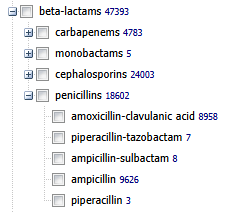
\includegraphics[width=0.45\textwidth]{figures/scope_broad_example}
\caption{Broad class hierarchy for beta-lactam antibiotics.}
\label{fig:broad-scope-example}
\end{figure}

\paragraph{Stage 4: model-ready table generation.}
After connection, the genotype evidence is converted into antibiotic-specific feature tables. These tables are the final inputs for XGBoost and for the rule-based baselines. Each table represents one modeling problem for one antibiotic under one biological scope, with one row per isolate.

\begin{figure}[H]
\centering
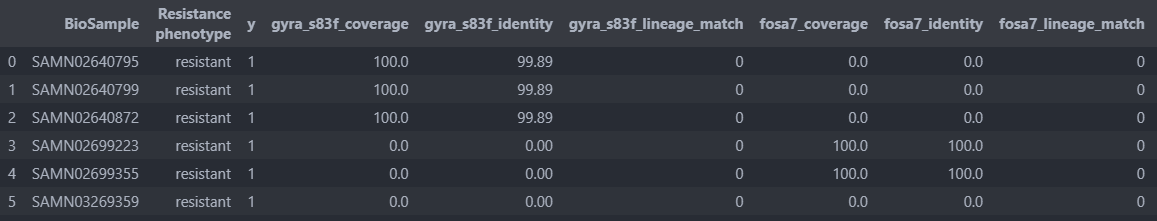
\includegraphics[width=0.9\textwidth]{figures/prepared_input_example}
\caption{Example of a prepared model-input table after genotype evidence has been aligned with phenotype labels.}
\label{fig:prepared-input-example}
\end{figure}

This staged construction separates data cleaning decisions from modeling decisions and makes each step easier to explain.

\subsection{Workflow Evolution}

Replace this section with your workflow evolution details.

\subsection{Workflow Execution}

Replace this section with your workflow execution details.


\newpage\cleardoublepage
\chapter{Chapter 4 Title}

\section{Experimental Results}

\subsection{Experimental setup}

The experiments are conducted on antibiotic-specific datasets prepared from the same shared genotype-phenotype cohort. The same cohort selection rules, phenotype cleaning rules, and genotype normalization rules are applied across all scopes to keep the comparison fair. The current implementation evaluates 14 antibiotics that satisfy the minimum sample and class-count thresholds required for stable supervised learning.

The main model-based comparison includes three determinant-connection scopes:

\begin{itemize}
    \item \textbf{Strict ML}
    \item \textbf{Broad ML}
    \item \textbf{All ML}
\end{itemize}

The direct genotype-to-phenotype baseline is implemented in two forms:

\begin{itemize}
    \item \textbf{Strict rule-based}
    \item \textbf{Broad rule-based}
\end{itemize}

This comparison is more meaningful for this bioinformatics study than comparing several generic classifiers because it isolates the effect of biological scope and prior knowledge.

\subsection{Average performance across methods}

Table~\ref{tab:method-average-metrics} summarizes the average performance of the five main method settings across the 14 antibiotics.

\begin{table}[H]
\centering
\caption{Average performance across antibiotics}
\label{tab:method-average-metrics}
\small
\begin{tabular}{lccccc}
\toprule
Method & Accuracy & Precision & Recall & ROC-AUC & Avg. zero rows \\
\midrule
Strict rule-based & 0.861 & 0.655 & 0.704 & -- & 4461.1 \\
Broad rule-based  & 0.839 & 0.648 & 0.987 & -- & 3790.5 \\
Strict ML         & 0.822 & 0.744 & 0.865 & 0.842 & 4461.1 \\
Broad ML          & 0.988 & 0.972 & 0.974 & 0.984 & 3790.5 \\
All ML            & 0.987 & 0.966 & 0.974 & 0.988 & 0.0 \\
\bottomrule
\end{tabular}
\end{table}

Several patterns are immediately visible. First, \textit{broad ML} and \textit{all ML} are the strongest overall settings, both achieving average accuracy near 0.99 and average recall around 0.974. Second, \textit{broad rule-based} has the highest average recall among the direct rule methods, reaching 0.987, but this comes with a clear loss in precision and specificity. Third, the \textit{strict} settings use a narrower biological scope but suffer from many zero-hit or zero-feature rows, especially for some beta-lactam antibiotics.

\subsection{Observed performance pattern of the ML scopes}

The model-based results show a clear overall pattern. The \textit{all} scope gives the best ability to separate resistant and susceptible isolates across antibiotics and removes the zero-feature problem completely. Its average ROC-AUC is 0.988, higher than the 0.984 achieved by \textit{broad ML} and much higher than the 0.842 of \textit{strict ML}. The \textit{broad} scope performs competitively for many antibiotics and is the strongest constrained alternative. The \textit{strict} scope is still useful as a narrow reference, but it is too fragile to serve as the default setting because it leaves too many isolates with no usable determinant evidence.

\begin{figure}[H]
\centering
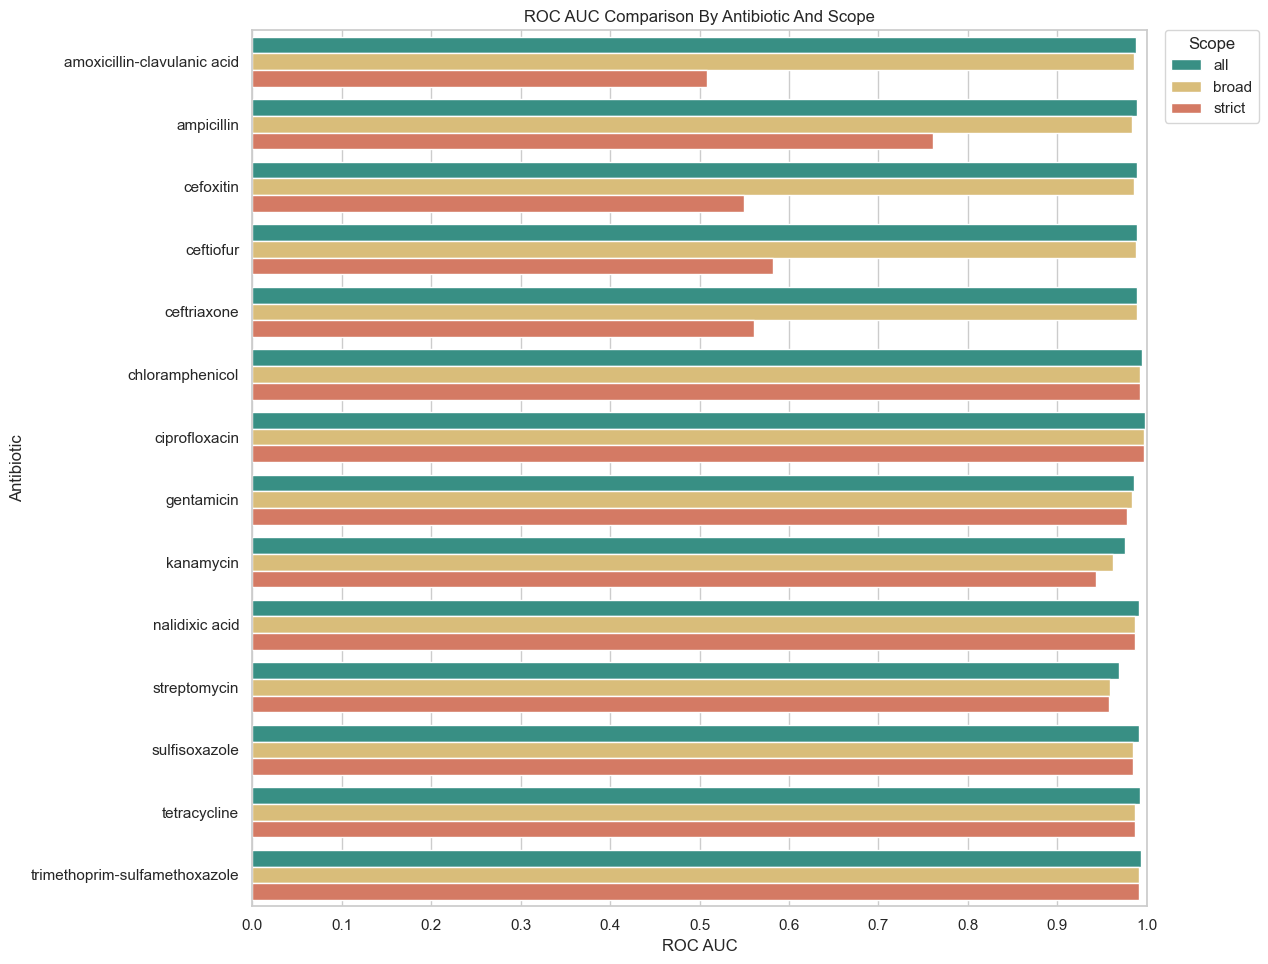
\includegraphics[width=0.95\textwidth]{figures/roc_auc_by_scope}
\caption{ROC-AUC comparison across antibiotics and determinant-connection scopes.}
\label{fig:roc-auc-by-scope}
\end{figure}

This pattern is biologically interpretable. Narrow matching improves feature specificity, but it can also exclude genes or mutations that are still useful within the same broader drug family. Relaxing the scope to \textit{broad} captures more same-class mechanisms, while the \textit{all} setting allows the model to use wider patterns among many detected determinants.

\subsection{Main result trends}

The results support four main conclusions:

\begin{enumerate}[label=\arabic*.]
    \item The \textit{all} scope is the strongest global default when the main objective is predictive performance.
    \item The \textit{broad} scope is the best compromise when interpretability is still important.
    \item The \textit{strict} scope is useful as a narrow biological baseline, but it fails on several antibiotics because the matching rule is too restrictive.
    \item Performance differences across antibiotics reflect real differences in resistance mechanism diversity and determinant coverage.
\end{enumerate}

\subsection{Rule-based versus machine-learning behavior}

The rule-based baselines are useful because they show when the presence of known determinants is already enough to predict phenotype and when machine learning adds real value. For some antibiotics, the direct rule is already very strong. For example, under the strict scope, ciprofloxacin reaches precision 0.968 and recall 0.998, chloramphenicol reaches precision 0.990 and recall 0.988, and nalidixic acid reaches precision 0.953 and recall 0.989. These results suggest that, for such antibiotics, the detected genes and mutations already match the phenotype closely.

However, the same direct rule becomes too weak or too coarse for other antibiotics. Under the strict rule baseline, ceftriaxone reaches recall only 0.101 and precision 0.090, while ceftiofur reaches recall 0.133 and precision 0.102. When the scope is relaxed to broad rule-based inference, recall for ceftriaxone increases sharply to 0.985, but precision remains only 0.489. This shows the main trade-off clearly: broader matching can recover missed resistant isolates, but it can also overcall resistance by accepting determinants that are related to the same drug class but are not specific enough to the target drug.

Machine learning changes this balance substantially. For ceftriaxone, \textit{broad ML} achieves precision 0.992 and recall 0.976, while \textit{all ML} achieves precision 0.990 and recall 0.974. In other words, the learned models keep the broad coverage needed to recover resistant isolates, but avoid much of the precision loss seen in broad rule-based inference. A similar pattern appears for ceftiofur and cefoxitin. These comparisons support the main scientific argument of the report: machine learning is most valuable when broader determinant evidence must be combined more carefully than a direct rule can do.

\subsection{Interpretation of zero-hit and zero-feature rows}

One of the clearest signals in the experiment is the role of zero rows. In the rule-based setting, a zero-hit row means that no determinant connected to the target antibiotic scope was found in the isolate. In the machine-learning setting, the corresponding zero-feature row means the model received an all-zero feature vector for that isolate. The averages in Table~\ref{tab:method-average-metrics} show that both strict settings suffer from roughly 4461 zero rows on average, whereas broad settings reduce this burden to about 3790 rows, and the all scope removes it entirely.

This result explains much of the performance gap between strict and broader settings. A narrow scope can be biologically conservative, but if it leaves too many isolates without usable determinant evidence, both rule-based prediction and machine learning start from a weak input.

\subsection{Discussion of limitations}

The current study predicts a binary resistant/susceptible phenotype rather than MIC, uses curated determinant resources rather than full pan-genome features, and has not yet performed external validation on an independent surveillance cohort. These limitations do not invalidate the study, but they define its scope clearly and position it as a determinant-based bioinformatics analysis rather than a full clinical deployment study.

\newpage\cleardoublepage
\chapter*{Conclusion}
\addcontentsline{toc}{chapter}{Conclusion}

Replace this chapter with your conclusion.
\newpage\cleardoublepage

\renewcommand{\bibname}{References}
\bibliography{references}\newpage\cleardoublepage

\end{document}
